\documentclass[10pt]{article}
\advance\hoffset by -0.7 truein\relax


\usepackage{graphicx}
%\input{epsf}

\topmargin=-0.4in
%\leftmargin=-1in 
\textwidth=6.3in
\textheight=8.8in


\usepackage{amssymb}
\usepackage{latexsym}
\usepackage{amsmath}
\usepackage{enumerate}
\usepackage{hyperref}
\usepackage{subcaption}

\usepackage{tikz}
\usepackage{pgfplots}

\begin{document}

\begin{figure}
  \centering
  
\includegraphics[width=0.25\textwidth]{images/simiam-round-logo.png}
\end{figure}

\title{{\huge{\bf{Sim.I.am: A Robot Simulator }}} \\
         Coursera: Control of Mobile Robots}
\author{Jean-Pierre de la Croix}
\date{Last Updated: \today}

\maketitle
\tableofcontents
\newpage
\section{Introduction}
This manual is going to be your resource for using the simulator with the programming assignments featured in the Coursera course, \textit{Control of Mobile Robots} (and included at the end of this manual). It will be updated from time to time whenever new features are added to the simulator or any corrections to the course material are made.

\subsection{Installation}

Download \texttt{simiam-coursera-week-X.zip} (where X is the corresponding week number for the assignment) from the course page on Coursera under \href{https://class.coursera.org/conrob-002/wiki/ProgrammingAssignments}{\textit{Programming Assignments}}. Make sure to download a new copy of the simulator \textbf{before} you start a new week's programming assignment, or whenever an announcement is made that a new version is available. It is important to stay up-to-date, since new versions may contain important bug fixes or features required for the programming assignment.

Unzip the \texttt{.zip} file to any directory.

\subsection{Requirements}

You will need a reasonably modern computer to run the robot simulator. While the simulator will run on hardware older than a Pentium 4, it will probably be a very slow experience. You will also need a copy of MATLAB. 

Thanks to support from MathWorks, a license for MATLAB and all required toolboxes is available to all students for the duration of the course. Check the \textit{Getting Started with MATLAB} section under \href{https://class.coursera.org/conrob-002/wiki/ProgrammingAssignments}{\textit{Programming Assignments}} on the course page for detailed instructions on how to download and install MATLAB on your computer.

\subsection{Bug Reporting}
If you run into a bug (issue) with the simulator, please create a post on the discussion forums in the \href{https://class.coursera.org/conrob-002/forum/list?forum_id=3}{\textit{Programming Assignments}} section. Make sure to leave a detailed description of the bug. Any questions or issues with MATLAB itself should be posted on the discussion forums in the \href{https://class.coursera.org/conrob-002/forum/list?forum_id=3}{\textit{MATLAB}} section.

\newpage
\section{Mobile Robot}

The mobile robot you will be working with in the programming exercises is the QuickBot. The QuickBot is equipped with five infrared (IR) range sensors, of which three are located in the front and two are located on its sides. The QuickBot has a two-wheel differential drive system (two wheels, two motors) with a wheel encoder for each wheel. It is powered by two 4x AA battery packs on top and can be controlled via software on its embedded Linux computer, the BeagleBone Black. You can build the QuickBot yourself by following the hardware lectures in this course.

\begin{figure}[t]
  \centering
  \begin{subfigure}{0.45\textwidth}
    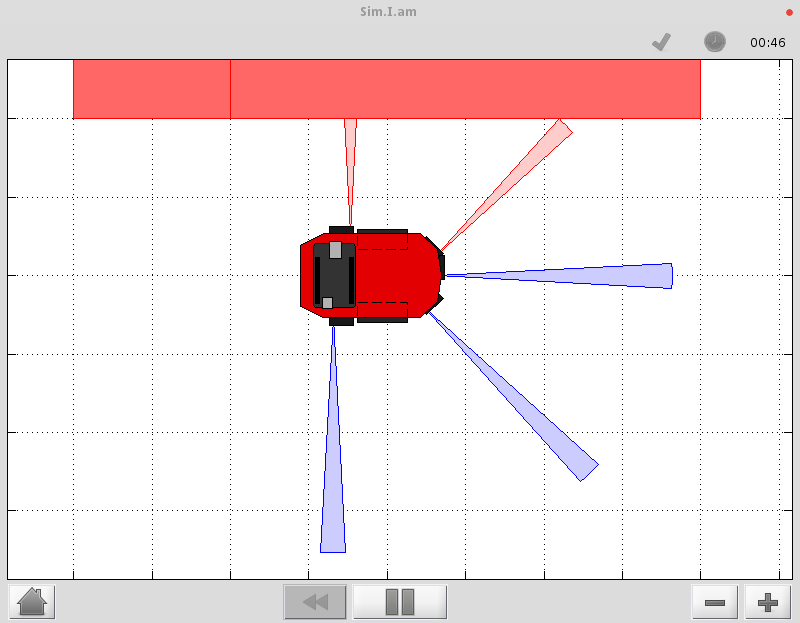
\includegraphics[width=\textwidth]{images/simiam-quickbot.png}
    \caption{Simulated QuickBot}
    \label{fig:simulated-quickbot}
  \end{subfigure}
  \begin{subfigure}{0.45\textwidth}
    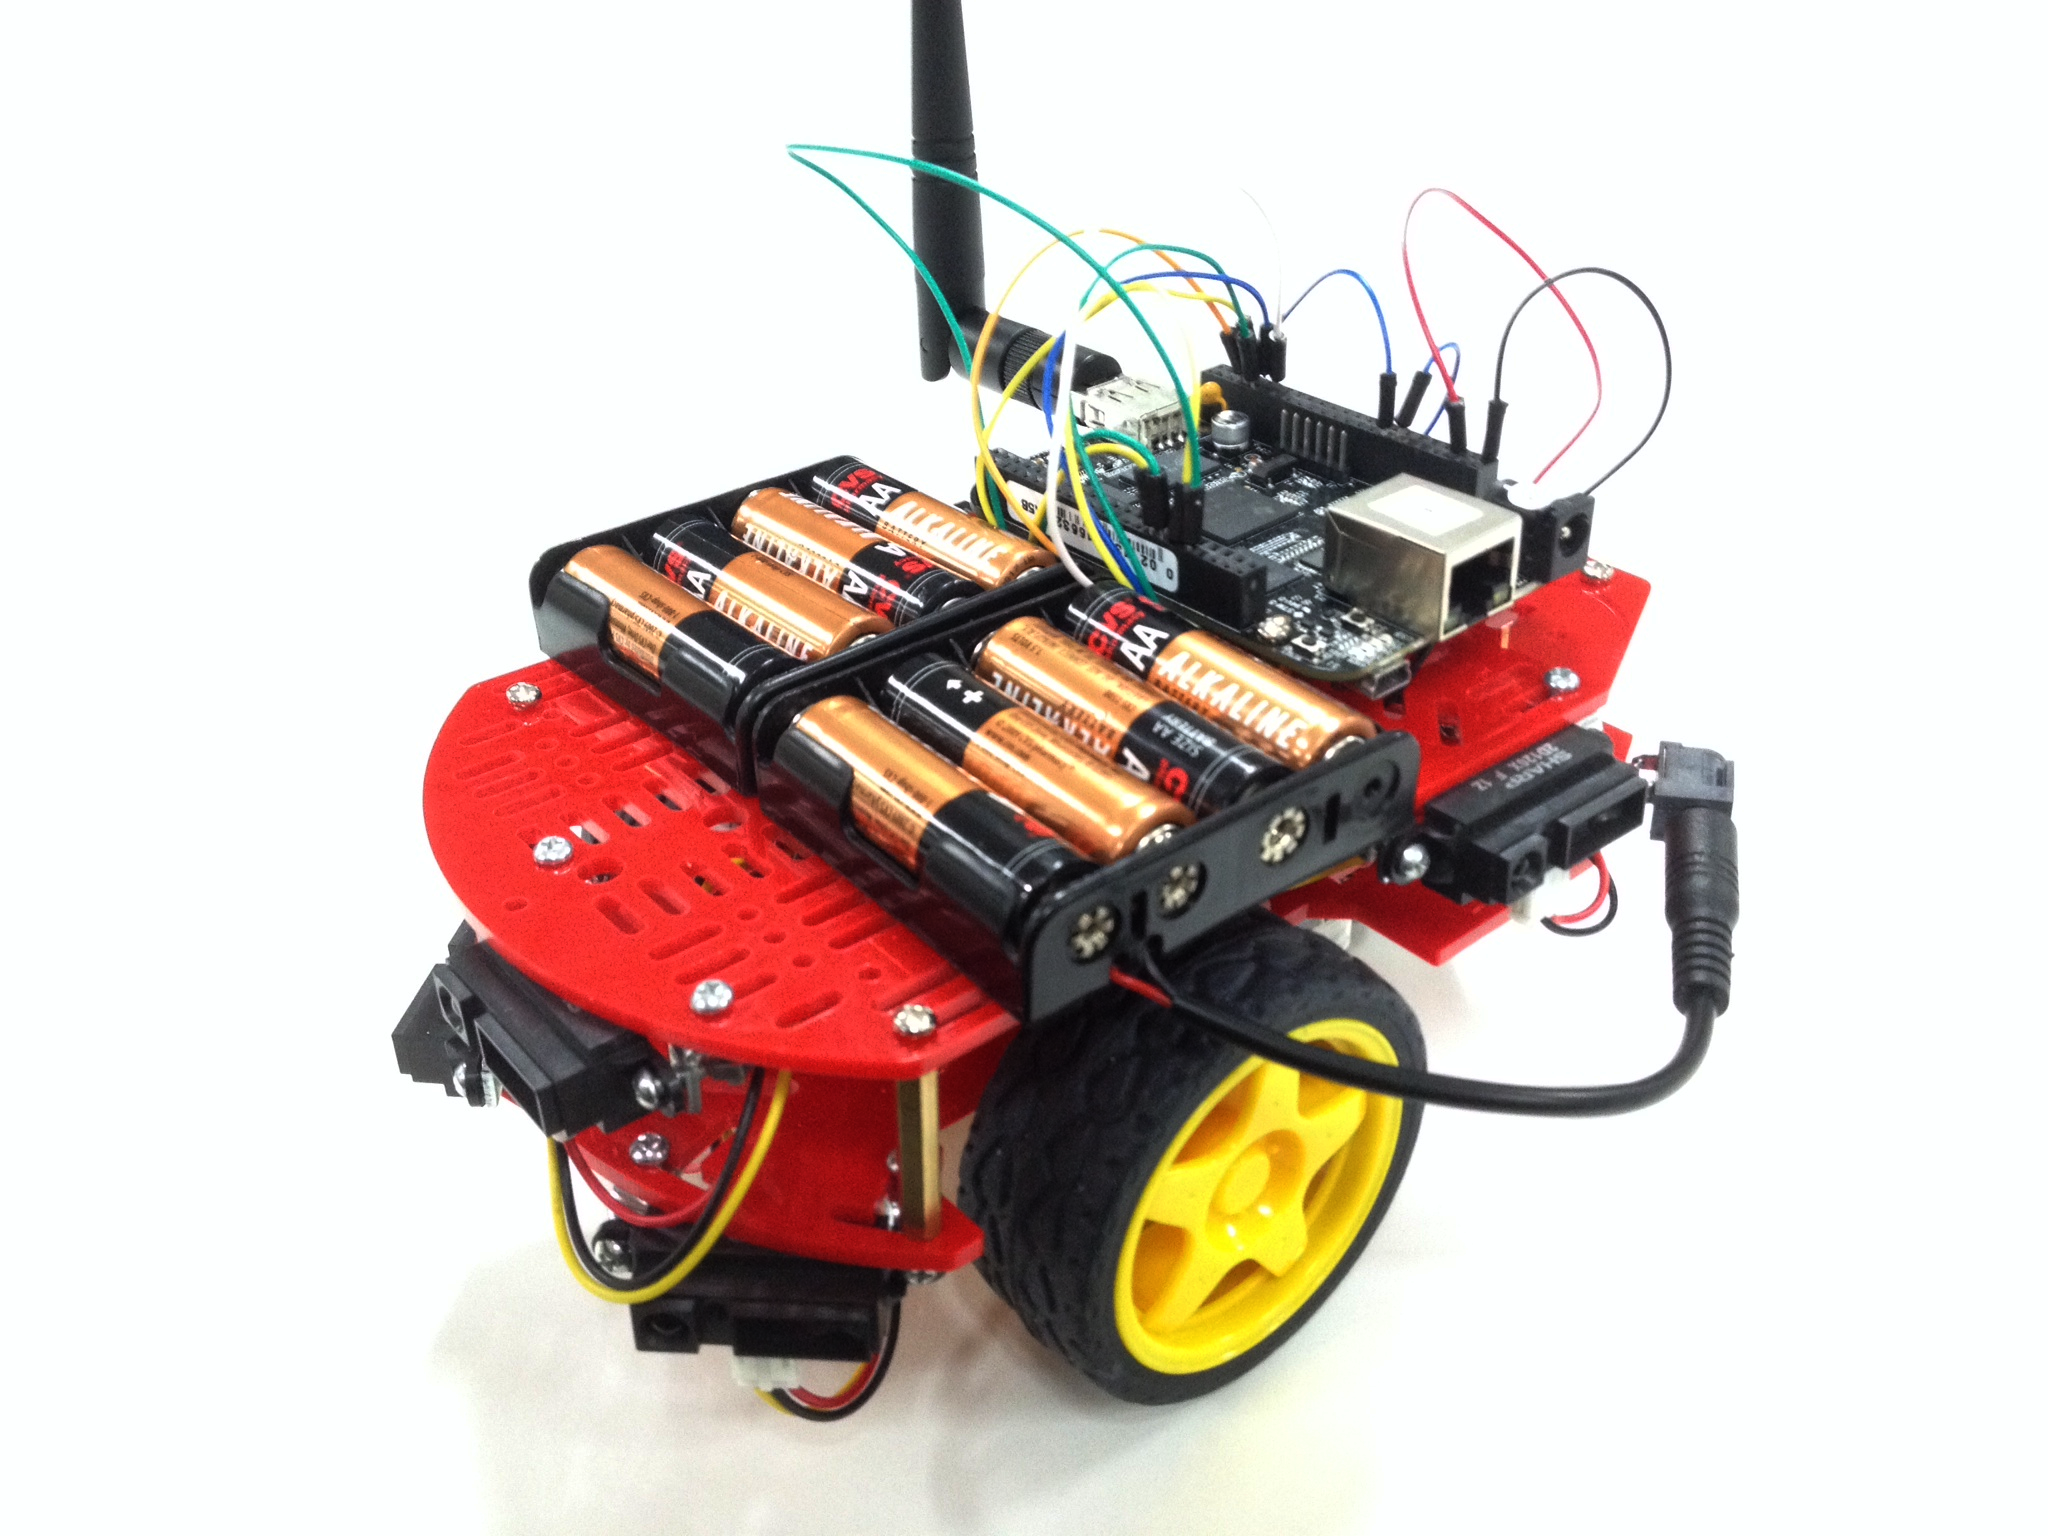
\includegraphics[width=\textwidth]{images/quickbot-red.png}
    \caption{Actual QuickBot}
    \label{fig:actual-quickbot}
  \end{subfigure}
  \caption{The QuickBot mobile robot in and outside of the simulator.}
  \label{fig:quickbot}
\end{figure}

Figure \ref{fig:quickbot} shows the simulated and actual QuickBot mobile robot. The robot simulator recreates the QuickBot as faithfully as possible. For example, the range, output, and field of view of the simulated IR range sensors match the specifications in the datasheet for the actual Sharp GP2D120XJ00F infrared proximity sensors on the QuickBot.

\subsection{IR Range Sensors}\label{irprox}
You will have access to the array of five IR sensors that encompass the QuickBot. The orientation (relative to the body of the QuickBot, as shown in figure \ref{fig:simulated-quickbot}) of IR sensors 1 through 5 is $90^\circ, 45^\circ, 0^\circ$, $-45^\circ, -90^\circ$, respectively.I R range sensors are effective in the range $0.04$ m to $0.3$ m only. However, the IR sensors return raw values in the range of $[0.4,2.75] V$ instead of the measured distances. Figure \ref{fig:ir-volts-meters} demonstrates the function that maps these sensors values to distances. To complicate matters slightly, the BeagleBone Black digitizes the analog output voltage using a voltage divider and a 12-bit, 1.8V analog-to-digital converter (ADC). Figure \ref{fig:ir-adc} is a look-up table to demonstrate the relationship between the ADC output, the analog voltage from the IR proximity sensor, and the approximate distance that corresponds to this voltage.

\begin{figure}[t]
  \centering
  \begin{subfigure}{0.45\textwidth}
    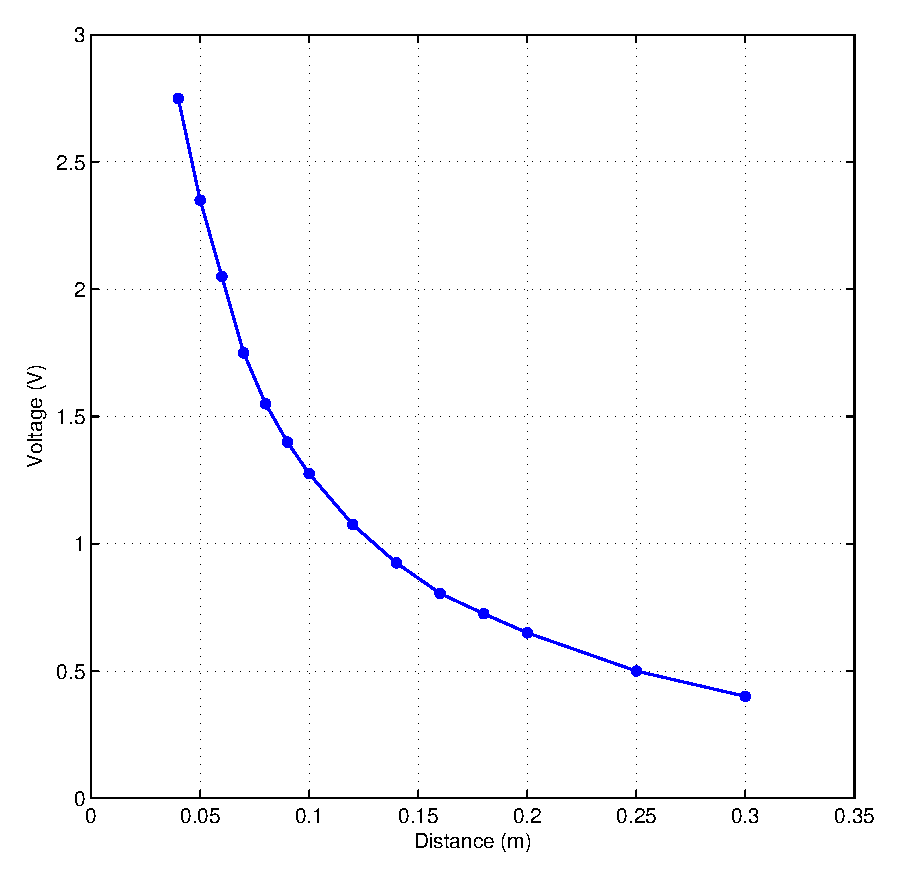
\includegraphics[width=\textwidth]{images/ir-sensor-graph.eps}
    \caption{Analog voltage output when an object is between 0.04m and 0.3m in the IR proximity sensor's field of view.}
    \label{fig:ir-volts-meters}
  \end{subfigure}
  $\qquad$
  \begin{subfigure}{0.45\textwidth}
    \begin{center}
    \begin{tabular}{|p{0.3\textwidth}|p{0.3\textwidth}|p{0.25\textwidth}|}
       \hline
       Distance (m) & Voltage (V) & ADC Out\\
       \hline
       0.04 & 2.750 & 917 \\
       0.05 & 2.350 & 783 \\
       0.06 & 2.050 & 683 \\
       0.07 & 1.750 & 583 \\
       0.08 & 1.550 & 517 \\
       0.09 & 1.400 & 467 \\
       0.10 & 1.275 & 425 \\
       0.12 & 1.075 & 358 \\
       0.14 & 0.925 & 308 \\
       0.16 & 0.805 & 268 \\
       0.18 & 0.725 & 242 \\
       0.20 & 0.650 & 217 \\
       0.25 & 0.500 & 167 \\
       0.30 & 0.400 & 133 \\
       \hline
    \end{tabular}
  \end{center}
    \caption{A look-up table for interpolating a distance (m) from the analog (and digital) output voltages.}
    \label{fig:ir-adc}
  \end{subfigure}
  \caption{A graph and a table illustrating the relationship between the distance of an object within the field of view of an infrared proximity sensor and the analog (and digital) ouptut voltage of the sensor.}
  \label{fig:quickbot}
\end{figure}

Any controller can access the IR array through the \texttt{robot} object that is passed into its \texttt{execute} function. For example,
\begin{verbatim}
  ir_distances = robot.get_ir_distances();
  for i=1:numel(robot.ir_array)
    fprintf('IR #%d has a value of %d', i, robot.ir_array(i).get_range());
    fprintf('or %0.3f meters.\n', ir_distances(i));
  end
\end{verbatim}

It is assumed that the function \texttt{get\_ir\_distances} properly converts from the ADC output to an analog output voltage, and then from the analog output voltage to a distance in meters. The conversion from ADC output to analog output voltage is simply,

\begin{equation*}
  V_{\text{ADC}} = \left\lfloor\frac{1000\cdot V_{\text{analog}}}{3}\right\rceil
\end{equation*}

\textbf{NOTE: For Week 2, the simulator uses a different voltage divider on the ADC; therefore, $V_{\text{ADC}}= V_{\text{analog}}*1000/2$. This has been fixed in subsequent weeks!}

Converting from the the analog output voltage to a distance is a little bit more complicated, because a) the relationships between analog output voltage and distance is not linear, and b) the look-up table provides a coarse sample of points on the curve in Figure \ref{fig:ir-volts-meters}. MATLAB has a \texttt{polyfit} function to fit a curve to the values in the look-up table, and a \texttt{polyval} function to interpolate a point on that fitted curve. The combination of the these two functions can be use to approximate a distance based on the analog output voltage. For more information, see Section \ref{sec:week-2}.

It is important to note that the IR proximity sensor on the actual QuickBot will be influenced by ambient lighting and other sources of interference. For example, under different ambient lighting conditions, the same analog output voltage may correspond to different distances of an object from the IR proximity sensor. This effect of ambient lighting (and other sources of noise) is \textbf{not} modelled in the simulator, but will be apparent on the actual hardware.

\subsection{Differential Wheel Drive}\label{diffdrive}
Since the QuickBot has a differential wheel drive (i.e., is not a unicyle), it has to be controlled by specifying the angular velocities of the right and left wheel $(v_r,v_l)$, instead of the linear and angular velocities of a unicycle $(v,\omega)$. These velocities are computed by a transformation from $(v,\omega)$ to $(v_r,v_\ell)$. Recall that the dynamics of the unicycle are defined as,
\begin{equation}
 \begin{split}
   \dot{x} &= vcos(\theta) \\
   \dot{y} &= vsin(\theta) \\
   \dot{\theta} &= \omega.
 \end{split}
\end{equation}
The dynamics of the differential drive are defined as,
\begin{equation}
 \begin{split}
  \dot{x} &= \frac{R}{2}(v_r+v_\ell)cos(\theta) \\
  \dot{y} &= \frac{R}{2}(v_r+v_\ell)sin(\theta) \\
  \dot{\theta} &= \frac{R}{L}(v_r-v_\ell),
 \end{split}
\end{equation}
where $R$ is the radius of the wheels and $L$ is the distance between the wheels.

The speed of the QuickBot can be set in the following way assuming that the \texttt{uni\_to\_diff} function has been implemented, which transforms $(v,\omega)$ to $(v_r,v_\ell)$:
\begin{verbatim}
 v = 0.15; % m/s
 w = pi/4; % rad/s
 % Transform from v,w to v_r,v_l and set the speed of the robot
 [vel_r, vel_l] = obj.robot.dynamics.uni_to_diff(robot,v,w);
 obj.robot.set_speeds(vel_r, vel_l);
\end{verbatim}

The maximum angular wheel velocity for the QuickBot is approximately 80 RPM or 8.37 rad/s. It is important to note that if the QuickBot is controlled ot move at maximum linear velocity, it is not possible to achieve any angular velocity, because the angular velocity of the wheel will have been maximized. Therefore, there exists a tradeoff between the linear and angular velocity of the QuickBot: \textit{the faster the robot should turn, the slower it has to move forward}.

\subsection{Wheel Encoders}

Each of the wheels is outfitted with a wheel encoder that increments or decrements a tick counter depending on whether the wheel is moving forward or backwards, respectively. Wheel encoders may be used to infer the relative pose of the robot. This inference is called \textbf{odometry}. The relevant information needed for odometry is the radius of the wheel ($32.5$mm), the distance between the wheels ($99.25$mm), and the number of ticks per revolution of the wheel ($16$ ticks/rev). For example,

\begin{verbatim}
 R = robot.wheel_radius; % radius of the wheel
 L = robot.wheel_base_length; % distance between the wheels
 tpr = robot.encoders(1).ticks_per_rev; % ticks per revolution for the right wheel

 fprintf('The right wheel has a tick count of %d\n', robot.encoders(1).state);
 fprintf('The left wheel has a tick count of %d\n', robot.encoders(2).state);
\end{verbatim}

For more information about odometry, see Section \ref{sec:week-2}.

\newpage
\section{Simulator}

Start the simulator with the \texttt{launch} command in MATLAB from the command window. It is important that this command is executed inside the unzipped folder (but not inside any of its subdirectories).

\begin{figure}[h]
  \centering
  \begin{subfigure}{0.45\textwidth}
    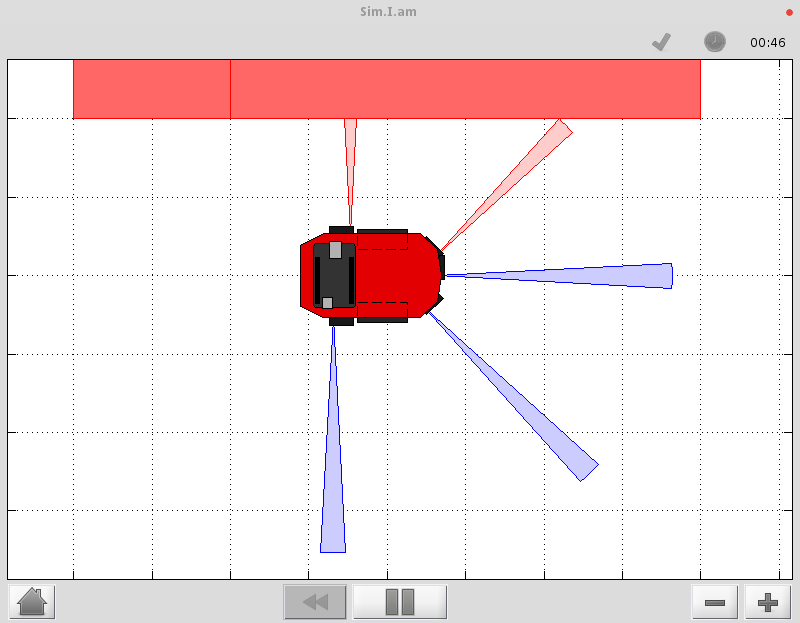
\includegraphics[width=\textwidth]{images/simiam-quickbot.png}
    \caption{Simulator}
    \label{fig:simulator}
  \end{subfigure}
  $\qquad$
  \begin{subfigure}{0.4\textwidth}
    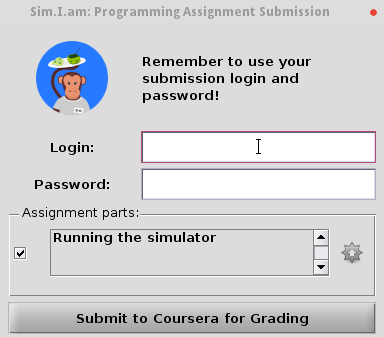
\includegraphics[width=\textwidth]{images/simiam-submit.png}
    \caption{Submission screen}
    \label{fig:submission}
  \end{subfigure}
  \caption{\texttt{launch} starts the simulator, while \texttt{submit} brings up the submission tool.}
  \label{fig:screens}
\end{figure}

Figure \ref{fig:simulator} is a screenshot of the graphical user interface (GUI) of the simulator. The GUI can be controlled by the bottom row of buttons. The first button is the \textit{Home} button and returns you to the home screen. The second button is the \textit{Rewind} button and resets the simulation. The third button is the \textit{Play} button, which can be used to play and pause the simulation. The set of \textit{Zoom} buttons or the mouse scroll wheel allows you to zoom in and out to get a better view of the simulation. Clicking, holding, and moving the mouse allows you to pan around the environment. You can click on a robot to follow it as it moves through the environment.

Figure \ref{fig:submission} is a screenshot of the submission screen. Each assignment can be submitted to Coursera for automatic grading and feedback. Start the submission tool by typing \texttt{submit} into the MATLAB command window. Use your login and password from the \href{https://class.coursera.org/conrob-002/assignment/list}{\textit{Assignments}} page. Your Coursera login and password will \textbf{not} work. Select which parts of the assignments in the list you would like to submit, then click \textit{Submit to Coursera for Grading}. You will receive feedback, either a green checkmark for pass, or a red checkmark for fail. If you receive a red checkmark, check the MATLAB command window for a helpful message.

\newpage
\section{Programming Assignments}

The following sections serve as a tutorial for getting through the simulator portions of the programming exercises. Places where you need to either edit or add code is marked off by a set of comments. For example,

\begin{verbatim}
  %% START CODE BLOCK %%
    [edit or add code here]
  %% END CODE BLOCK %%
\end{verbatim}

To start the simulator with the \texttt{launch} command from the command window, it is important that this command is executed inside the unzipped folder (but not inside any of its subdirectories).

\subsection{Week 1}

This week's exercises will help you learn about MATLAB and robot simulator:

\begin{enumerate}
\item Since the assignments in this course involve programming in MATLAB, you should familiarize yourself with MATLAB (both the environment and the language). Review the resources posted in the "Getting Started with MATLAB" section on the \href{https://class.coursera.org/conrob-002/wiki/ProgrammingAssignments}{\textit{Programming Assignments}} page.

\item Familiarize yourself with the simulator by reading this manual and downloading the robot simulator posted on the \href{https://class.coursera.org/conrob-002/wiki/ProgrammingAssignments}{\textit{Programming Assignments}} section on the Coursera page.
\end{enumerate}

\subsection{Week 2}
\label{sec:week-2}
Start by downloading the robot simulator for this week from the \href{https://class.coursera.org/conrob-002/assignment/view?assignment_id=5}{Week 2 programming assignment}. Before you can design and test controllers in the simulator, you will need to implement three components of the simulator:

\begin{enumerate}
 \item Implement the transformation from unicycle dynamics to differential drive dynamics, i.e. convert from $(v,\omega)$ to the right and left \textbf{angular} wheel speeds $(v_r,v_l)$.
 
 In the simulator, $(v,\omega)$ corresponds to the variables \texttt{v} and \texttt{w}, while $(v_r,v_l)$ correspond to the variables \texttt{vel\_r} and \texttt{vel\_l}. The function used by the controllers to convert from unicycle dynamics to differential drive dynamics is located in \texttt{+simiam/+robot/+dynamics/DifferentialDrive.m}. The function is named \texttt{uni\_to\_diff}, and inside of this function you will need to define \texttt{vel\_r} ($v_r$) and \texttt{vel\_l} ($v_l$) in terms of \texttt{v}, \texttt{w}, \texttt{R}, and \texttt{L}. \texttt{R} is the radius of a wheel, and \texttt{L} is the distance separating the two wheels. Make sure to refer to Section \ref{diffdrive} on ``Differential Wheel Drive'' for the dynamics.
 
 \item Implement odometry for the robot, such that as the robot moves around, its pose $(x,y,\theta)$ is estimated based on how far each of the wheels have turned. Assume that the robot starts at (0,0,0).
 
 The tutorial located at \url{www.orcboard.org/wiki/images/1/1c/OdometryTutorial.pdf} covers how odometry is computed. The general idea behind odometry is to use wheel encoders to measure the distance the wheels have turned over a small period of time, and use this information to approximate the change in pose of the robot.

 The pose of the robot is composed of its position $(x,y)$ and its orientation $\theta$ on a 2 dimensional plane (\textbf{note}: the video lecture may refer to robot's orientation as $\phi$). The currently estimated pose is stored in the variable \texttt{state\_estimate}, which bundles \texttt{x} ($x$), \texttt{y} ($y$), and \texttt{theta} ($\theta$). The robot updates the estimate of its pose by calling the \texttt{update\_odometry} function, which is located in \texttt{+simiam/+controller/+quickbot/QBSupervisor.m}. This function is called every \texttt{dt} seconds, where \texttt{dt} is $0.033$s (or a little more if the simulation is running slower).
 \begin{verbatim}  
  % Get wheel encoder ticks from the robot
  right_ticks = obj.robot.encoders(1).ticks;
  left_ticks = obj.robot.encoders(2).ticks;

  % Recall the wheel encoder ticks from the last estimate
  prev_right_ticks = obj.prev_ticks.right;
  prev_left_ticks = obj.prev_ticks.left;

  % Previous estimate 
  [x, y, theta] = obj.state_estimate.unpack();

  % Compute odometry here
  R = obj.robot.wheel_radius;
  L = obj.robot.wheel_base_length;
  m_per_tick = (2*pi*R)/obj.robot.encoders(1).ticks_per_rev;\end{verbatim}
  The above code is already provided so that you have all of the information needed to estimate the change in pose of the robot. \texttt{right\_ticks} and \texttt{left\_ticks} are the accumulated wheel encoder ticks of the right and left wheel. \texttt{prev\_right\_ticks} and \texttt{prev\_left\_ticks} are the wheel encoder ticks of the right and left wheel saved during the last call to \texttt{update\_odometry}. \texttt{R} is the radius of each wheel, and \texttt{L} is the distance separating the two wheels. \texttt{m\_per\_tick} is a constant that tells you how many meters a wheel covers with each tick of the wheel encoder. So, if you were to multiply \texttt{m\_per\_tick} by (\texttt{right\_ticks}-\texttt{prev\_right\_ticks}), you would get the distance travelled by the right wheel since the last estimate.
  
  Once you have computed the change in $(x,y,\theta)$ (let us denote the changes as \texttt{x\_dt}, \texttt{y\_dt}, and \texttt{theta\_dt}) , you need to update the estimate of the pose:
  \begin{verbatim}
    theta_new = theta + theta_d;
    x_new = x + x_dt;
    y_new = y + y_dt;\end{verbatim}
 
 \item Read the "IR Range Sensors" section in the manual and take note of the table in Figure \ref{fig:ir-adc}, which maps distances (in meters) to raw IR values. Implement code that converts raw IR values to distances (in meters).
 
 To retrieve the distances (in meters) measured by the IR proximity sensor, you will need to implement a conversion from the raw IR values to distances in the \texttt{get\_ir\_distances} function located in \texttt{+simiam/+robot/Quickbot.m}.
 \begin{verbatim}
  function ir_distances = get_ir_distances(obj)
      ir_array_values = obj.ir_array.get_range();
      ir_voltages = ir_array_values;
      coeff = [];
      ir_distances = polyval(coeff, ir_voltages);
  end\end{verbatim}
  The variable \texttt{ir\_array\_values} is an array of the IR raw values. Divide this array by $500$ to compute the \texttt{ir\_voltages} array. The \texttt{coeff} should be the coefficients returned by
  \begin{verbatim}
    coeff = polyfit(ir_voltages_from_table, ir_distances_from_table, 5);\end{verbatim}
where the first input argument is an array of IR voltages from the table in Figure \ref{fig:ir-adc} and the second argument is an array of the corresponding distances from the table in Figure \ref{fig:ir-adc}. The third argument specifies that we will use a fifth-order polynomial to fit to the data. Instead of running this fit every time, execute the polyfit once in the MATLAB command line, and enter them manually on the third line, i.e. \texttt{coeff = [ ... ];}. If the coefficients are properly computed, then the last line will use polyval to convert from IR voltages to distances using a fifth-order polynomial using the coefficients in \texttt{coeff}. 
 
\end{enumerate}

\subsubsection*{How to test it all}

To test your code, the simulator will is set to run a single P-regulator that will steer the robot to a particular angle (denoted $\theta_d$ or, in code, \texttt{theta\_d}). This P-regulator is implemented in \texttt{+simiam/+controller/} \texttt{GoToAngle.m}. If you want to change the linear velocity of the robot, or the angle to which it steers, edit the following two lines in \texttt{+simiam/+controller/+quickbot/QBSupervisor.m}
 \begin{verbatim}
  obj.theta_d = pi/4;
  obj.v = 0.1; %m/s\end{verbatim}
\begin{enumerate}
  \item To test the transformation from unicycle to differential drive, first set \texttt{obj.theta\_d=0}. The robot should drive straight forward. Now, set \texttt{obj.theta\_d} to positive or negative $\frac{\pi}{4}$. If positive, the robot should start off by turning to its left, if negative it should start off by turning to its right. \textbf{Note}: If you haven't implemented odometry yet, the robot will just keep on turning in that direction.
  \item To test the odometry, first make sure that the transformation from unicycle to differential drive works correctly. If so, set \texttt{obj.theta\_d} to some value, for example $\frac{\pi}{4}$, and the robot's P-regulator should steer the robot to that angle. You may also want to uncomment the \texttt{fprintf} statement in the \texttt{update\_odometry} function to print out the current estimate position to see if it make sense. Remember, the robot starts at $(x,y,\theta)=(0,0,0)$.
  \item To test the IR raw to distances conversion, edit \texttt{+simiam/+controller/}\texttt{GoToAngle.m} and uncomment the following section:
  \begin{verbatim}
  % for i=1:numel(ir_distances)
  %   fprintf('IR %d: %0.3fm\n', i, ir_distances(i));
  % end\end{verbatim}
  This \texttt{for} loop will print out the IR distances. If there are no obstacles (for example, walls) around the robot, these values should be close (if not equal to) $0.3$m. Once the robot gets within range of a wall, these values should decrease for some of the IR sensors (depending on which ones can sense the obstacle). \texttt{Note:} The robot will eventually collide with the wall, because we have not designed an obstacle avoidance controller yet!
\end{enumerate}

\subsection{Week 3}

Start by downloading the new robot simulator for this week from the \href{}{Week 3 programming assignment}. This week you will be implementing the different parts of a PID regulator that steers the robot successfully to some goal location. This is known as the go-to-goal behavior:

\begin{enumerate}
 \item Calculate the heading (angle), $\theta_g$, to the goal location $(x_g,y_g)$. Let $u$ be the vector from the robot located at $(x,y)$ to the goal located at $(x_g,y_g)$, then $\theta_g$ is the angle $u$ makes with the $x$-axis (positive $\theta_g$ is in the counterclockwise direction).

All parts of the PID regulator will be implemented in the file \texttt{+simiam/+controller/GoToGoal.m}. Take note that each of the three parts is commented to help you figure out where to code each part. The vector $u$ can be expressed in terms of its $x$-component, $u_x$, and its $y$-component, $u_y$. $u_x$ should be assigned to \texttt{u\_x} and $u_y$ to \texttt{u\_y} in the code. Use these two components and the \texttt{atan2} function to compute the angle to the goal, $\theta_g$ (\texttt{theta\_g} in the code).


 \item Calculate the error between $\theta_g$ and the current heading of the robot, $\theta$.
 
 The error \texttt{e\_k} should represent the error between the heading to the goal \texttt{theta\_g} and the current heading of the robot \texttt{theta}. Make sure to use \texttt{atan2} and/or other functions to keep the error between $[-\pi,\pi]$.
 
 \item Calculate the proportional, integral, and derivative terms for the PID regulator that steers the robot to the goal.
 
 As before, the robot will drive at a constant linear velocity \texttt{v}, but it is up to the PID regulator to steer the robot to the goal, i.e compute the correct angular velocity \texttt{w}. The PID regulator needs three parts implemented:
 
  \begin{enumerate}[(i)]
    \item The first part is the proportional term \texttt{e\_P}. It is simply the current error \texttt{e\_k}. \texttt{e\_P} is multiplied by the proportional gain \texttt{obj.Kp} when computing \texttt{w}.
    \item The second part is the integral term \texttt{e\_I}. The integral needs to be approximated in discrete time using the total accumulated error \texttt{obj.E\_k}, the current error \texttt{e\_k}, and the time step \texttt{dt}. \texttt{e\_I} is multiplied by the integral gain \texttt{obj.Ki} when computing \texttt{w}, and is also saved as \texttt{obj.E\_k} for the next time step.
    \item The third part is the derivative term \texttt{e\_D}. The derivative needs to be approximated in discrete time using the current error \texttt{e\_k}, the previous error \texttt{obj.e\_k\_1}, and the the time step \texttt{dt}. \texttt{e\_D} is multiplied by the derivative gain \texttt{obj.Kd} when computing \texttt{w}, and the current error \texttt{e\_k} is saved as the previous error \texttt{obj.e\_k\_1} for the next time step.
  \end{enumerate}
  
  Now, you need to tune your PID gains to get a fast settle time ($\theta$ matches $\theta_g$ within $10\%$ in three seconds or less) and there should be little overshoot (maximum $\theta$ should not increase beyond $10\%$ of the reference value $\theta_g$). What you don't want to see are the following two graphs when the robot tries to reach goal location $(x_g,y_g)=(0,-1)$:
  
\begin{figure}[h]
  \centering
  \begin{subfigure}{0.45\textwidth}
    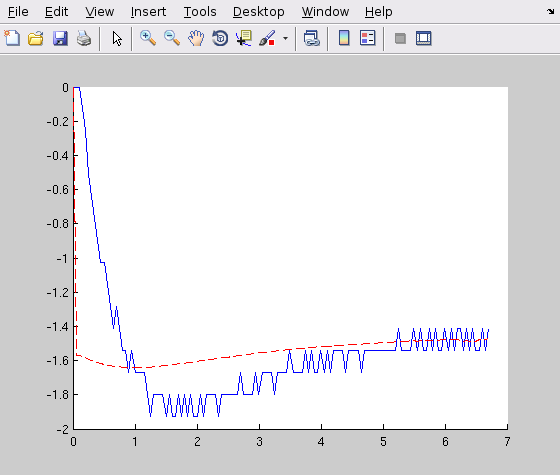
\includegraphics[width=\textwidth]{images/week-3-pid-overshoot.png}
    \caption{Overshoot}
    \label{fig:pid-overshoot}
  \end{subfigure}
  $\qquad$
  \begin{subfigure}{0.45\textwidth}
    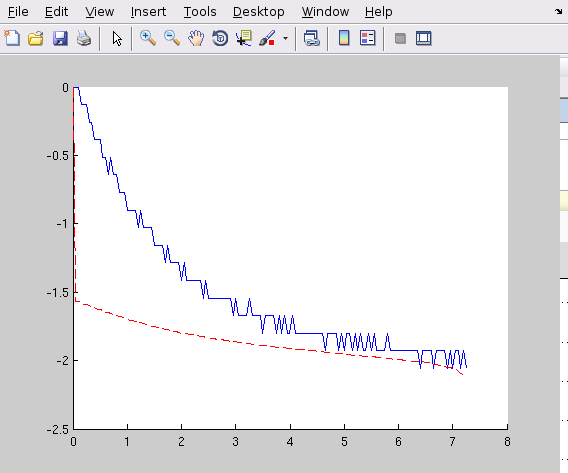
\includegraphics[width=\textwidth]{images/week-3-pid-undershoot.png}
    \caption{Undershoot (slow settle time)}
    \label{fig:pid-undershoot}
  \end{subfigure}
  \caption{PID gains were picked poorly, which lead to overshoot and poor settling times.}
  \label{fig:screens}
\end{figure}

Figure \ref{fig:pid-undershoot} demonstrates undershoot, which could be fixed by increasing the proportional gain or adding some integral gain for better tracking. Picking better gains leads to the graph in Figure \ref{fig:pid-normal}.

\begin{figure}[h]
  \centering
  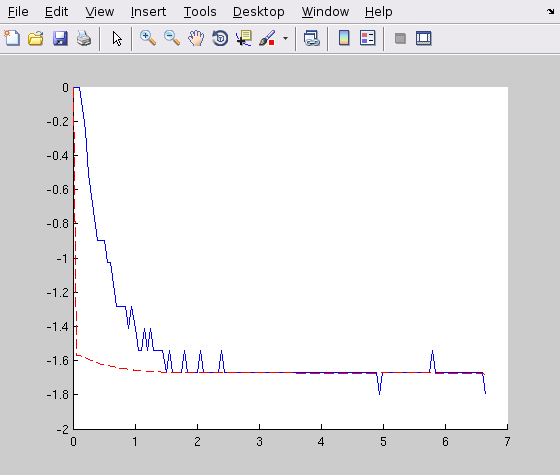
\includegraphics[width=0.5\textwidth]{images/week-3-pid-normal.png}
  \caption{Faster settle time and good tracking with little overshoot.}
  \label{fig:pid-normal}
\end{figure}

  
  \item Ensure that the robot steers with an angular velocity $\omega$, even if the combination of $v$ and $\omega$ exceeds the maximum angular velocity of the robot's motors.
  
  This week we'll tackle the first of two limitations of the motors on the QuickBot. The first limitation is that the robot's motors have a maximum angular velocity, and the second limitation is that the motors stall at low speeds. We will discuss the latter limitation in a later week and focus our attention on the first limitation. Suppose that we pick a linear velocity $v$ that requires the motors to spin at $90\%$ power. Then, we want to change $\omega$ from $0$ to some value that requires $20\%$ more power from the right motor, and $20\%$ less power from the left motor. This is not an issue for the left motor, but the right motor cannot turn at a capacity greater than $100\%$. The results is that the robot cannot turn with the $\omega$ specified by our controller.
  
  Since our PID controllers focus more on steering than on controlling the linear velocity, we want to prioritize $\omega$ over $v$ in situations, where we cannot satisfy $\omega$ with the motors. In fact, we will simply reduce $v$ until we have sufficient headroom to achieve $\omega$ with the robot. The function \texttt{ensure\_w} in \texttt{+simiam/+controller/+quickbot/QBSupervisor.m} is designed ensure that $\omega$ is achieved even if the original combination of $v$ and $\omega$ exceeds the maximum $v_r$ and $v_l$.
  
  Complete \texttt{ensure\_w}. Suppose $v_{r,d}$ and $v_{l,d}$ are the angular wheel velocities needed to achieve $\omega$. Then \texttt{vel\_rl\_max} is $\max(v_{r,d},v_{l,d})$ and \texttt{vel\_rl\_min} is $\min(v_{r,d},v_{l,d})$. A motor's maximum forward angular velocity is \texttt{obj.robot.max\_vel} (or $\text{vel}_{\max}$). So, for example, the equation that represents the \texttt{if/else} statement for the right motors is:
  \begin{equation*}
    v_r= 
\begin{cases}
    v_{r,d} - (\max(v_{r,d},v_{l,d})-vel_{\max})& \text{if } \max(v_{r,d},v_{l,d}) > vel_{\max}\\
    v_{r,d} - (\min(v_{r,d},v_{l,d})+vel_{\max})& \text{if } \min(v_{r,d},v_{l,d}) < -vel_{\max}\\
    v_{r,d},              & \text{otherwise},
\end{cases}
  \end{equation*}
  which defines the appropriate $v_r$ (or \texttt{vel\_r}) needed to achieve $\omega$. This equation also applies to computing a new $v_l$. The results of \texttt{ensures\_w} is that if $v$ and $\omega$ are so large that $v_r$ and/or $v_l$ exceed $\text{vel}_{\max}$, then $v$ is scaled back to ensure $\omega$ is achieved (Note: $\omega$ is precapped at the beginnging of \texttt{ensure\_w} to the maximum $\omega$ possible if the robot is stationary).
  
\end{enumerate}

\subsection*{How to test it all}

To test your code, the simulator is set up to use the PID regulator in \texttt{GoToGoal.m} to drive the robot to a goal location and stop. If you want to change the linear velocity of the robot, the goal location, or the distance from the goal the robot will stop, then edit the following three lines in \texttt{+simiam/+controller/} \texttt{+quickbot/QBSupervisor.m}.
  \begin{verbatim}
    obj.goal = [-1,1];
    obj.v = 0.2;
    obj.d_stop = 0.05;\end{verbatim}
Make sure the goal is located inside the walls, i.e. the $x$ and $y$ coordinates of the goal should be in the range $[-1,1]$. Otherwise the robot will crash into a wall on its way to the goal!

\begin{enumerate}
  \item To test the heading to the goal, set the goal location to \texttt{obj.goal = [1,1]}. \texttt{theta\_g} should be approximately $\frac{\pi}{4} \approx 0.785$ initially, and as the robot moves forward (since $v=0.1$ and $\omega=0$) \texttt{theta\_g} should increase. Check it using a \texttt{fprintf} statment or the plot that pops up. \texttt{theta\_g} corresponds to the red dashed line (i.e., it is the reference signal for the PID regulator).
  \item Test this part with the implementation of the third part.
  \item To test the third part, run the simulator and check if the robot drives to the goal location and stops. In the plot, the blue solid line (\texttt{theta}) should match up with the red dashed line (\texttt{theta\_g}). You may also use \texttt{fprintf} statements to verify that the robot stops within \texttt{obj.d\_stop} meters of the goal location.
  \item To test the fourth part, set \texttt{obj.v=10}. Then add the following two lines of code after the call to \texttt{ensure\_w} in the \texttt{execute} function of \texttt{QBSupervisor.m}.
  \begin{verbatim}
    [v_limited, w_limited] = obj.robot.dynamics.diff_to_uni(vel_r, vel_l);
    fprintf('(v,w) = (%0.3f,%0.3f), (v_limited,w_limited) = (%0.3f, %0.3f)\n', ...
                                      outputs.v, outputs.w, v_limited, w_limited);
  \end{verbatim}
   If $\omega\neq\omega_{\text{limited}}$, then $\omega$ is not ensured by \texttt{ensure\_w}. This function should scale back $v$, such that it is possible for the robot to turn with the $\omega$ output by the controller (unless $|\omega|>5.48$ rad/s).
\end{enumerate}

\subsection*{How to migrate your solutions from last week.}

Here are a few pointers to help you migrate your own solutions from last week to this week's simulator code. You only need to pay attention to this section if you want to use your own solutions, otherwise you can use what is provided for this week and skip this section.

\begin{enumerate}
 \item You may overwrite \texttt{+simiam/+robot/+dynamics/DifferentialDrive.m} with your own version from last week.
 \item You should not overwrite \texttt{+simiam/+robot/QuickBot.m} with your own version from last week! Many changes were made to this file for this week.
 \item You should not overwrite \texttt{+simiam/+controller/+quickbot/QBSupervisor.m}! However, to use your own solution to the odometry, you can replace the provided \texttt{update\_odometry} function in \texttt{K3Supervisor.m} with your own version from last week.
\end{enumerate}

\subsection{Week 4}

Start by downloading the new robot simulator for this week from the Week 4 programming assignment. This week you will be implementing the different parts of a controller that steers the robot successfully away from obstacles to avoid a collision. This is known as the avoid-obstacles behavior. The IR sensors allow us to measure the distance to obstacles in the environment, but we need to compute the points in the world to which these distances correspond.
\begin{figure}[h]
 \centering
 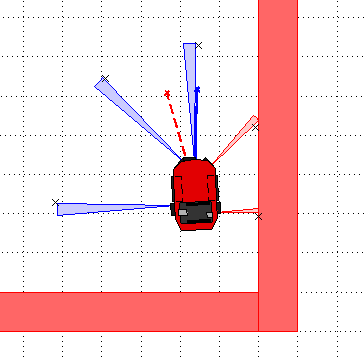
\includegraphics[scale=0.5]{images/week-4-ir-points.png}
 \caption{IR range to point transformation.}
  \label{fig:week4irpoints}
\end{figure}
Figure \ref{fig:week4irpoints} illustrates these points with a black cross. The strategy for obstacle avoidance that we will use is as follows:

\begin{enumerate}
  \item Transform the IR distances to points in the world.
  \item Compute a vector to each point from the robot, $u_1,u_2,\ldots,u_9$.
  \item Weigh each vector according to their importance, $\alpha_1u_1,\alpha_2u_2,\ldots,\alpha_9u_9$. For example, the front and side sensors are typically more important for obstacle avoidance while moving forward.
  \item Sum the weighted vectors to form a single vector, $u_{ao}=\alpha_1u_1+\ldots+\alpha_9u_9$.
  \item Use this vector to compute a heading and steer the robot to this angle.
\end{enumerate}

This strategy will steer the robot in a direction with the most free space (i.e., it is a direction \textit{away} from obstacles). For this strategy to work, you will need to implement three crucial parts of the strategy for the obstacle avoidance behavior:

\begin{enumerate}
  \item Transform the IR distance (which you converted from the raw IR values in Week 2) measured by each sensor to a point in the reference frame of the robot.
  
  A point $p_i$ that is measured to be $d_i$ meters away by sensor $i$ can be written as the vector (coordinate) $v_i=\begin{bmatrix}d_i \\ 0\end{bmatrix}$ in the reference frame of sensor $i$. We first need to transform this point to be in the reference frame of the robot. To do this transformation, we need to use the pose (location and orientation) of the sensor in the reference frame of the robot: $(x_{s_i},y_{s_i},\theta_{s_i})$ or in code, \texttt{(x\_s,y\_s,theta\_s)}. The transformation is defined as:
  
  \begin{equation*}
    v'_i = R(x_{s_i},y_{s_i},\theta_{s_i})\begin{bmatrix}v_i \\ 1\end{bmatrix},
  \end{equation*}
  where $R$ is known as the transformation matrix that applies a translation by $(x,y)$ and a rotation by $\theta$:
  \begin{equation*}
    R(x,y,\theta) = \begin{bmatrix}\cos(\theta) & -\sin(\theta) & x \\ 
                                   \sin(\theta) &  \cos(\theta) & y \\
                                             0 &            0 & 1\end{bmatrix},
  \end{equation*}
  which you need to implement in the function \texttt{obj.get\_transformation\_matrix}.
  
  In \texttt{+simiam/+controller/+AvoidObstacles.m}, implement the transformation in the \texttt{apply\_sensor} \texttt{\_geometry} function. The objective is to store the transformed points in \texttt{ir\_distances\_rf}, such that this matrix has $v'_1$ as its first column, $v'_2$ as its second column, and so on.
  
  \item Transform the point in the robot's reference frame to the world's reference frame.
  
  A second transformation is needed to determine where a point $p_i$ is located in the world that is measured by sensor $i$. We need to use the pose of the robot, $(x,y,\theta)$, to transform the robot from the robot's reference frame to the world's reference frame. This transformation is defined as:
  
  \begin{equation*}
    v''_i = R(x,y,\theta)v'_i
  \end{equation*}
  
  In \texttt{+simiam/+controller/+AvoidObstacles.m}, implement this transformation in the \texttt{apply\_sensor} \texttt{\_geometry} function. The objective is to store the transformed points in \texttt{ir\_distances\_wf}, such that this matrix has $v''_1$ as its first column, $v''_2$ as its second column, and so on. This matrix now contains the coordinates of the points illustrated in Figure \ref{fig:week4irpoints} by the black crosses. Note how these points \textit{approximately} correspond to the distances measured by each sensor (Note: \textit{approximately}, because of how we converted from raw IR values to meters in Week 2).
  
  \item Use the set of transformed points to compute a vector that points away from the obstacle. The robot will steer in the direction of this vector and successfully avoid the obstacle.
  
  In the function \texttt{execute} implement parts 2.-4. of the obstacle avoidance strategy.
  \begin{enumerate}[(i)]
    \item Compute a vector $u_i$ to each point (corresponding to a particular sensor) from the robot. Use a point's coordinate from \texttt{ir\_distances\_wf} and the robot's location (\texttt{x},\texttt{y}) for this computation.
    \item Pick a weight $\alpha_i$ for each vector according to how important you think a particular sensor is for obstacle avoidance. For example, if you were to multiply the vector from the robot to point $i$ (corresponding to sensor $i$) by a small value (e.g., $0.1$), then sensor $i$ will not impact obstacle avoidance significantly. Set the weights in \texttt{sensor\_gains}. \textbf{Note}: Make sure to that the weights are symmetric with respect to the left and right sides of the robot. Without any obstacles around, the robot should only steer slightly right (due to a small asymmetry in the how the IR sensors are mounted on the robot).
    \item Sum up the weighted vectors, $\alpha_iu_i$, into a single vector $u_{ao}$.
    \item Use $u_ao$ and the pose of the robot to compute a heading that steers the robot away from obstacles (i.e., in a direction with free space, because the vectors that correspond to directions with large IR distances will contribute the most to $u_{ao}$).    
  \end{enumerate} 
\end{enumerate}

\subsection*{QuickBot Motor Limitations}

Last week we implemented a function, \texttt{ensure\_w}, which was responsible for respecting $\omega$ from the controller as best as possible by scaling $v$ if necessary. This implementation assumed that it was possible to control the angular velocity in the range $[-\text{vel}_{\max},\text{vel}_{\max}]$. This range reflected the fact that the motors on the QuickBot have a maximum rotational speed. However, it is also true that the motors have a minimum speed before the robot starts moving. If not enough power is applied to the motors, the angular velocity of a wheel remains at $0$. Once enough power is applied, the wheels spin at a speed $\text{vel}_{\min}$.

The \texttt{ensure\_w} function has been updated this week to take this limitation into account. For example, small $(v,\omega)$ may not be achievable on the QuickBot, so \texttt{ensure\_w} scales up $v$ to make $\omega$ possible. Similarily, if $(v,\omega)$ are both large, \texttt{ensure\_w} scales down $v$ to ensure $\omega$ (as was the case last week). You can uncomment the two \texttt{fprintf} statements to see $(v,\omega)$ before and after.

There is nothing that needs to be added or implemented for this week in \texttt{ensure\_w}, but you may find it interesting how one deals with physical limitations on a mobile robot, like the QuickBot. This particular approach has an interesting consequence, which is that if $v>0$, then $v_r$ and $v_l$ are both positive (and vice versa, if $v<0$). Therefore, we often have to increase or decrease $v$ significantly to ensure $\omega$ even if it were better to make small adjustments to both $\omega$ and $v$. As with most of the components in these programming assignments, there are alternative designs with their own advantages and disadvantages. Feel free to share your designs with everyone on the discussion forums!

\subsection*{How to test it all}

To test your code, the simulator is set up to use load the \texttt{AvoidObstacles.m} controller to drive the robot around the environment without colliding with any of the walls. If you want to change the linear velocity of the robot, then edit the following line in \texttt{+simiam/+controller/}\texttt{+quickbot/QBSupervisor.m}.
  \begin{verbatim}
    obj.v = 0.2;\end{verbatim}

Here are some tips on how to test the three parts:

\begin{enumerate}
  \item Test the first part with the second part.
  \item Once you have implemented the second part, one black cross should match up with each sensor as shown in Figure \ref{fig:week4irpoints}. The robot should drive forward and collide with the wall. The blue line indicates the direction that the robot is currently heading ($\theta$).
  \item Once you have implemented the third part, the robot should be able to successfully navigate the world without colliding with the walls (obstacles). If no obstacles are in range of the sensors, the red line (representing $u_ao$) should just point forward (i.e., in the direction the robot is driving). In the presence of obstacles, the red line should point away from the obstacles in the direction of free space.
\end{enumerate}

You can also tune the parameters of the PID regulator for $\omega$ by editing \texttt{obj.Kp}, \texttt{obj.Ki}, and \texttt{obj.Kd} in \texttt{AvoidObstacles.m}. The PID regulator should steer the robot in the direction of $u_ao$, so you should see that the blue line tracks the red line. \textbf{Note:} The red and blue lines (as well as, the black crosses) will likely deviate from their positions on the robot. The reason is that they are drawn with information derived from the odometry of the robot. The odometry of the robot accumulates error over time as the robot drives around the world. This odometric drift can be seen when information based on odometry is visualized via the lines and crosses. 

\subsection*{How to migrate your solutions from last week}

Here are a few pointers to help you migrate your own solutions from last week to this week's simulator code. You only need to pay attention to this section if you want to use your own solutions, otherwise you can use what is provided for this week and skip this section.

\begin{enumerate}
 \item You may overwrite the same files as listed for Week 3.
 \item You may overwrite \texttt{+simiam/+controller/GoToGoal.m} with your own version from last week.
 \item You should not overwrite \texttt{+simiam/+controller/+quickbot/QBSupervisor.m}! However, to use your own solution to the odometry, you can replace the provided \texttt{update\_odometry} function in \texttt{QBSupervisor.m} with your own version from last week.
 \item You may replace the PID regulator in \texttt{+simiam/+controller/AvoidObstacles.m} with your own version from the previous week (i.e., use the PID code from \texttt{GoToGoal.m}).
\end{enumerate}

\subsection{Week 5}
Start by downloading the new robot simulator for this week from the Week 5 assignment. This week you will be adding small improvements to  testing two arbitration mechanisms: blending and hard switches. Arbitration between the two controllers will allow the robot to drive to a goal, while not colliding with any obstacles on the way.

\begin{enumerate}
  \item Implement a simple control for the linear velocity, $v$, as a function of the angular velocity, $\omega$. Add it to both \texttt{+simiam/+controller/GoToGoal.m} and \texttt{+simiam/+controller/AvoidObstacles.m}.
  
  So far, we have implemented controllers that either steer the robot towards a goal location, or steer the robot away from an obstacle. In both cases, we have set the linear velocity, $v$, to a constant value of $0.1$ m/s or similar. While this approach works, it certainly leave plenty of room for improvement. We will improve the performance of both the go-to-goal and avoid-obstacles behavior by dynamically adjusting the linear velocity based on the angular velocity of the robot.
  
We previously learned that with a differential drive robot, we cannot, for example, drive the robot at the maximum linear and angular velocities. Each motor has a maximum and minimum angular velocity; therefore, there must be a trade-off between linear and angular velocities: linear velocity has to decrease in some cases for angular velocity to increase, and vice versa.
  
  We added the \texttt{ensure\_w} function over the last two weeks, which ensured that $\omega$ is achieved by scaling $v$. However, for example, one could improve the above strategy by letting the linear velocity be a function of the angular velocity \textit{and} the distance to the goal (or distance to the nearest obstacle).
  
  Improve your go-to-goal and avoid-obstacles controllers by adding a simple function that adjusts $v$ as function of $\omega$ and other information. For example, the linear velocity in the go-to-goal controller could be scaled by $\omega$ and the distance to the goal, such that the robot slows down as it reaches the goal. 
  
  \textbf{Note}: This part of the programming assignment is open ended and not checked by the automatic grader, but it will help with the other parts of this assignment.
  
  \item Combine your go-to-goal controller and avoid-obstacle controller into a single controller that blends the two behaviors. Implement it in \texttt{+simiam/+controller/AOandGTG.m}.
  
  It's time to implement the first type of arbitration mechanism between multiple controllers: \textit{blending}. The solutions to the go-to-goal and avoid-obstacles controllers have been combined into a single controller, \texttt{+simiam/+controller/AOandGTG.m}. However, one important piece is missing. \texttt{u\_gtg} is a vector pointing to the goal from the robot, and \texttt{u\_ao} is a vector pointing from the robot to a point in space away from obstacles. These two vectors need to be combined (blended) in some way into the vector \texttt{u\_ao\_gtg}, which should be a vector that points the robot both away from obstacles and towards the goal.
  
  The combination of the two vectors into \texttt{u\_ao\_gtg} should result in the robot driving to a goal without colliding with any obstacles in the way. Do not use \texttt{if/else} to pick between \texttt{u\_gtg} or \texttt{u\_ao}, but rather think about weighing each vector according to their importance, and then linearly combining the two vectors into a single vector, \texttt{u\_ao\_gtg}. For example,
  \begin{eqnarray*}
    \alpha &=& 0.75 \\
    u_{\text{ao,gtg}} &=& \alpha u_{\text{gtg}}+(1-\alpha)u_{\text{ao}}
  \end{eqnarray*}
  In this example, the go-to-goal behavior is stronger than the avoid-obstacle behavior, but that \textit{may} not be the best strategy. $\alpha$ needs to be carefully tuned (or a different weighted linear combination needs to be designed) to get the best balance between go-to-goal and avoid-obstacles. To make life easier, consider using the normalized versions of $u_{\text{gtg}}$ and $u_{\text{ao}}$ defined in the video lecture.
  
  \item Implement the switching logic that switches between the go-to-goal controller and the avoid-obstacles controller, such that the robot avoids any nearby obstacles and drives to the goal when clear of any obstacles.
  
  The second type of arbitration mechanism is \textit{switching}. Instead of executing both go-to-goal and avoid-obstacles simultaneously, we will only execute one controller at a time, but switch between the two controllers whenever a certain condition is satisfied.
  
  In the \texttt{execute} function of \texttt{+simiam/+controller/+khepera3/K3Supervisor.m}, you will need to implement the switching logic between go-to-goal and avoid-obstacles. The supervisor has been extended since last week to support switching between different controllers (or states, where a state simply corresponds to one of the controllers being executed). In order to switch between different controllers (or states), the supervisor also defines a set of events. These events can be checked to see if they are true or false. The idea is to start of in some state (which runs a certain controller), check if a particular event has occured, and if so, switch to a new controller.
  
  The tools that you should will need to implement the switching logic:
  \begin{enumerate}[(i)]
    \item Four events can be checked with the \texttt{obj.check\_event(name)} function, where \texttt{name} is the name of the state:
      \begin{itemize}
        \item \texttt{`at\_obstacle'} checks to see if any of front sensors (all but the three IR sensors in the back of the robot) detect an obstacle at a distance less than \texttt{obj.d\_at\_obs}. Return \texttt{true} if this is the case, \texttt{false} otherwise.
        \item \texttt{`at\_goal'} checks to see if the robot is within \texttt{obj.d\_stop} meters of the goal location.
        \item \texttt{`unsafe'} checks to see if any of the front sensors detect an obstacle at a distance less than \texttt{obj.d\_unsafe}.
        \item \texttt{`obstacle\_cleared'} checks to see if all of the front sensors report distances greater than \texttt{obj.d\_at\_obs} meters.
      \end{itemize}
    \item The \texttt{obj.switch\_state(name)} function switches between the states/controllers. There currently are four possible values that \texttt{name} can be:
      \begin{itemize}
        \item \texttt{`go\_to\_goal'} for the go-to-goal controller.
        \item \texttt{`avoid\_obstacles'} for the avoid-obstacles controller.
        \item \texttt{`ao\_and\_gtg'} for the blending controller.
        \item \texttt{`stop'} for stopping the robot.
      \end{itemize}
  \end{enumerate}
  
  Implement the logic for switching to \texttt{avoid\_obstacles}, when \texttt{at\_obstacle} is true, switching to \texttt{go\_to\_goal} when \texttt{obstacle\_cleared} is true, and switching to \texttt{stop} when \texttt{at\_goal} is true. 
  
  
  \textbf{Note:} Running the blending controller was implemented using these switching tools as an example. In the example, \texttt{check\_event('at\_goal')} was used to switch from \texttt{ao\_and\_gtg} to \texttt{stop} once the robot reaches the goal.
  
  \item Improve the switching arbitration by using the blended controller as an intermediary between the go-to-goal and avoid-obstacles controller.
  
  The blending controller's advantage is that it (hopefully) smoothly blends go-to-goal and avoid-obstacles together. However, when there are no obstacle around, it is better to purely use go-to-goal, and when the robot gets dangerously close, it is better to only use avoid-obstacles. The switching logic performs better in those kinds of situations, but jitters between go-to-goal and avoid-obstacle when close to a goal. A solution is to squeeze the blending controller in between the go-to-goal and avoid-obstacle controller.
  
  Implement the logic for switching to \texttt{ao\_and\_gtg}, when \texttt{at\_obstacle} is true, switching to \texttt{go\_to\_goal} when \texttt{obstacle\_cleared} is true, switching to \texttt{avoid\_obstacles} when \texttt{unsafe} is true, and switching to \texttt{stop} when \texttt{at\_goal} is true.
\end{enumerate}

\subsubsection*{How to test it all}

To test your code, the simulator is set up to either use the blending arbitration mechanism or the switching arbitration mechanism. If \texttt{obj.is\_blending} is \texttt{true}, then blending is used, otherwise switching is used. 

Here are some tips to the test the four parts:

\begin{enumerate}
  \item Test the first part with the second part. Uncomment the line:\begin{verbatim}
      fprintf('(v,w) = (%0.3f,%0.3f)\n', outputs.v, outputs.w);\end{verbatim}
    It is located with the code for the blending, which you will test in the next part. Watch \texttt{(v,w)} to make sure your function works as intended.
  \item Test the second part by setting \texttt{obj.is\_blending} to \texttt{true}. The robot should successfully navigate to the goal location $(1,1)$ without colliding with the obstacle that is in the way. Once the robot is near the goal, it should stop (you can adjust the stopping distance with \texttt{obj.d\_stop}). The output plot will likely look something similar to (depends on location of obstacles, and how the blending is implemented):
    \begin{figure}[h]
 \centering
 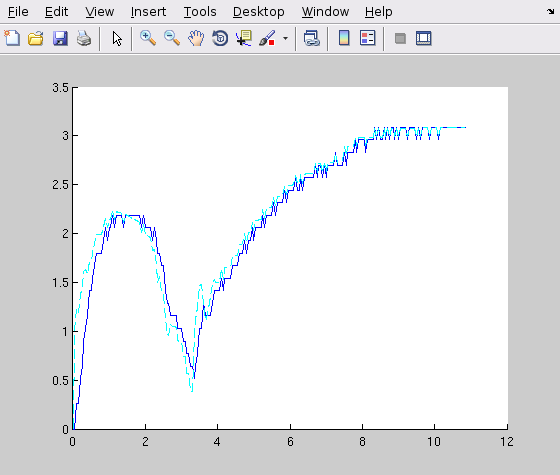
\includegraphics[scale=0.5]{images/week-5-part-2.png}
%  \caption{IR range to point transformation.}
  \label{fig:week5part2}
\end{figure}
  \item Test the third part by setting \texttt{obj.is\_blending} to \texttt{false}. The robot should successfully navigate to the same goal location $(1,1)$ without colliding with the obstacle that is in the way. Once the robot is near the goal, it should stop. The output plot will likely look something similar to:
    \begin{figure}[h!]
 \centering
 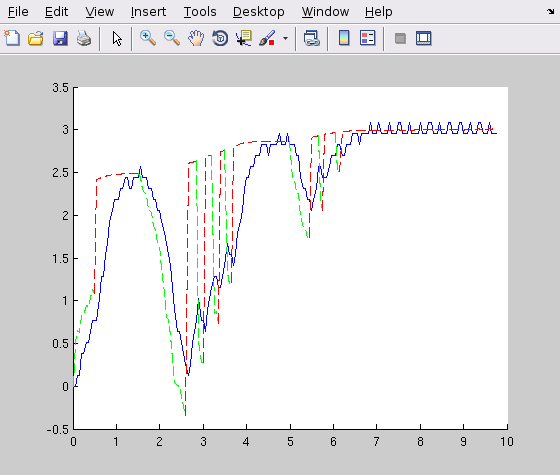
\includegraphics[scale=0.5]{images/week-5-part-3.png}
%  \caption{IR range to point transformation.}
  \label{fig:week5part3}
\end{figure}\newpage
  
  Notice that the blue line is the current heading of the robot, the red line is the heading set by the go-to-goal controller, and the green line is the heading set by the avoid-obstacles controller. You should see that the robot switches frequently between the two during its journey. Also, you will see messages in the MATLAB window stating that a switch has occurred.
  
  \item Test the fourth part in the same way as the third part. This time, the output plot will likely look something similar to:
  \begin{figure}[h]
 \centering
 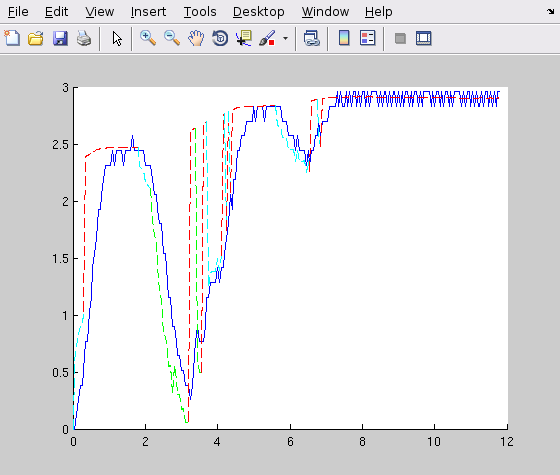
\includegraphics[scale=0.5]{images/week-5-part-4.png}
%  \caption{IR range to point transformation.}
  \label{fig:week5part4}
\end{figure}
  
  Notice that the controller still switches, but less often than before, because it now switches to the blended controller (cyan line) instead. Depending on how you set \texttt{obj.d\_unsafe} and \texttt{obj.d\_at\_obs}, the number of switches and between which controllers the supervisor switches may change. Experiment with different settings to observe their effect.
    
\end{enumerate}

\subsubsection*{How to migrate your solutions from last week}
Here are a few pointers to help you migrate your own solutions from last week to this week's simulator code. You only need to pay attention to this section if you want to use your own solutions, otherwise you can use what is provided for this week and skip this section.

\begin{enumerate}
 \item The simulator has seen a significant amount of changes from last week to support this week's programming exercises. It is \textbf{recommended} that you do not overwrite any of the files this week with your solutions from last week.
 \item However, you can selectively replace the sections delimited last week (by \texttt{START/END CODE BLOCK}) in \texttt{GoToGoal.m} and \texttt{AvoidObstacles.m}, as well as the sections that were copied from each into \texttt{AOandGTG.m}.
\end{enumerate}

\end{document}
